            
\documentclass{beamer}
\usepackage{beamerthemeshadow,graphicx,amsfon    ts, amsmath, mhchem}
\begin{document}
\title{Effects of Hydroxyl Radical Chemistry on Methane Emissions Estimates}
\author{Newton Nguyen}
% \date{May 4, 2016}
% Slide 1
\frame{\titlepage} 

% \frame{\frametitle{Table of contents}\tableofcontents} 


% Slide 2
\frame{\frametitle{Methane Overview}
  \begin{center}
    \begin{tabular}{c c}
      \includegraphics[width=0.4\textwidth]{test2.pdf} &
                                                         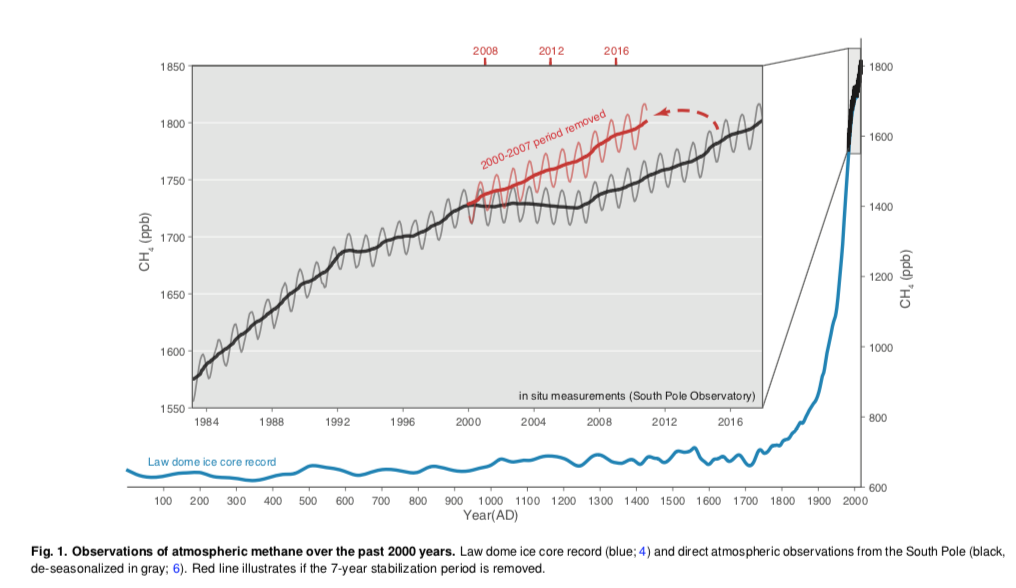
\includegraphics[width=0.4\textwidth]{methane_timeseries.png} 
    \end{tabular}
  \end{center}
  \begin{itemize}
  \item Second strongest anthropogenic greenhouse gas 
  \item Precursor to tropospheric ozone 
  \end{itemize}
}

% Slide 3
\frame{\frametitle{Constraining the Methane Sink}
  \begin{center}
    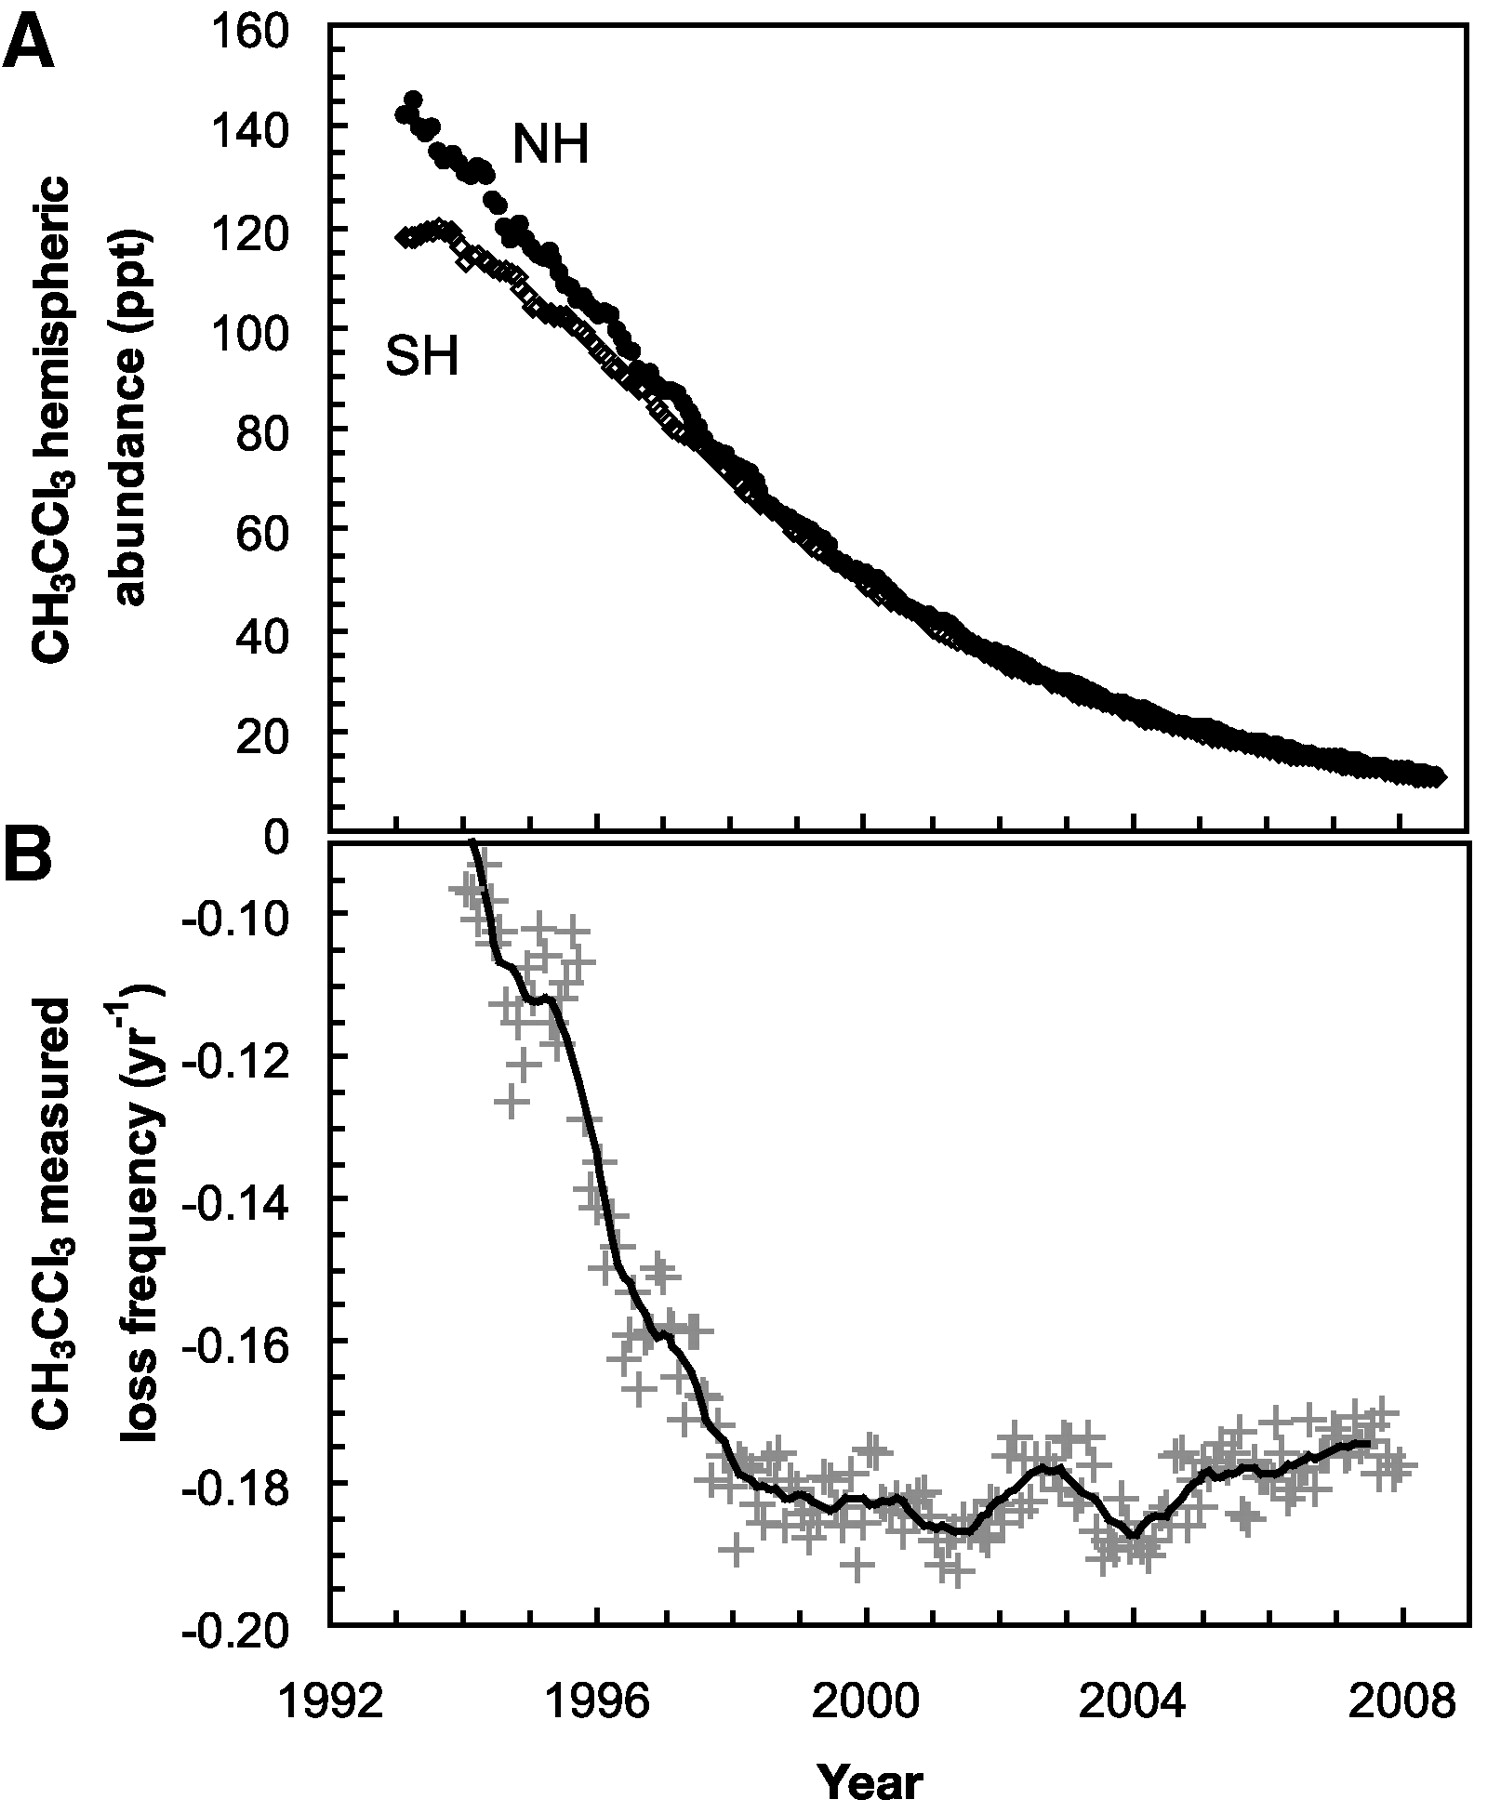
\includegraphics[width=0.3\textwidth]{Montzka2011-F1.jpg}
  \end{center}
  \begin{itemize}
  \item The Hydroxyl Radical (OH) is the main sink of methane in the troposphere
  \item OH is produced through photolysis
  \item MCF is used as a proxy for OH
  \end{itemize}
}

% Slide 4
\frame{\frametitle{The Box Model Approach}
  \begin{center}
    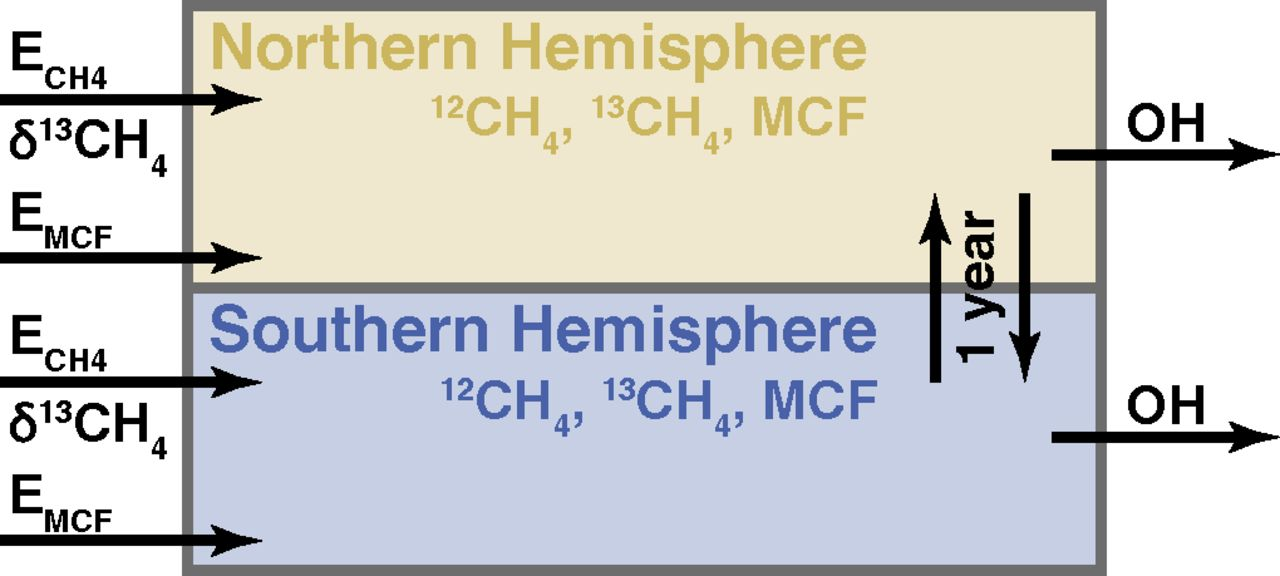
\includegraphics[scale=0.4]{Turner2017-F1.jpg}
  \end{center}
}

% Slide 5
\frame{\frametitle{Most Likely Solution}
  \begin{center}
    % \begin{tabular}
    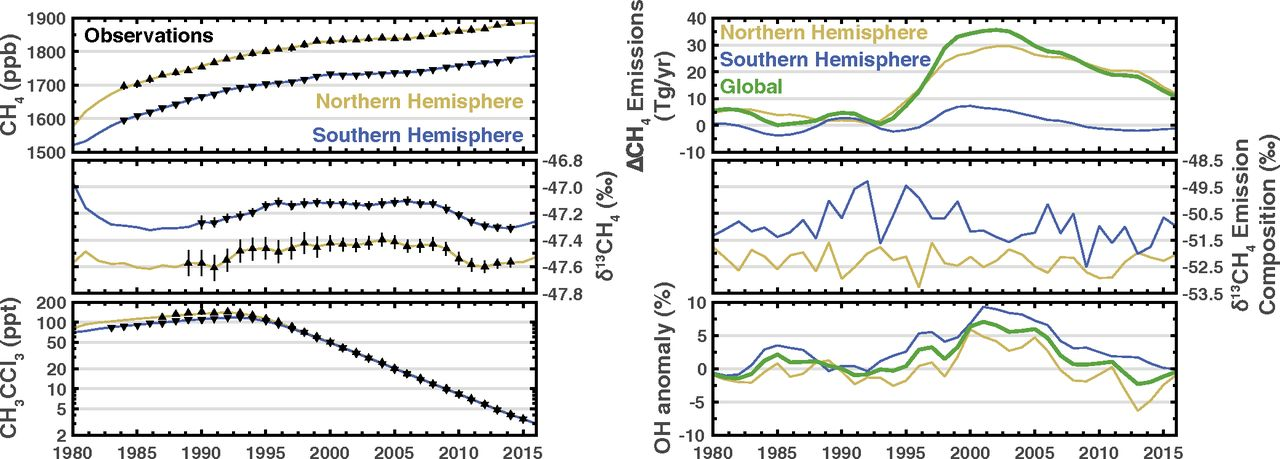
\includegraphics{Turner2017-F2.jpg} \\
    \begin{equation}
      \frac{d[CH_4]}{dt}=S_{CH_4}-k_1[CH_4][OH] 
    \end{equation}
    % \end{tabular}
  \end{center}
  \begin{itemize}
  \item Inverted for $S_{CH_4}$ based on observed $[CH_4]$ and infered values of [OH]
  \item Most likely solution is a 25 Tg/yr decrease in $S_{CH_4}$ with a 7\% decrease in [OH]
  \item Ignores variable lifetime of \ce{CH4} due to interactive chemistry. What are the resulting biases?
  \end{itemize}
}

% Slide 6
\frame{\frametitle{Chemical System}
  \begin{align*}
    OH + CH_4 \Longrightarrow (multiple steps) \Longrightarrow CO + products \\
    OH + CO \Longrightarrow CO_2 + H \\
    OH + X \Longrightarrow products 
  \end{align*}

  \begin{align*}
    R_1 = k_1 [OH] [CH_4] \\
    R_2 = k_2 [OH] [CO] \\
    R_3 = k_3 [OH] [X] 
  \end{align*}
  \begin{itemize}
  \item $R_i$ is reaction rate (loss of reactants)
  \item $K_i$ reaction rate constant (impirically obtained)
  \item [x] represents other sinks of OH 
  \end{itemize}
}

% Slide 7
\frame{\frametitle{The System of Equations}
  \begin{align*}
    R_1 = k_1 [OH] [CH_4] \\
    R_2 = k_2 [OH] [CO] \\ 
    R_3 = k_3 [OH] [X]
  \end{align*}
  \begin{align*}
    \frac{d[CH_4]}{dt} = SCH_4 - R_1 \\
    \frac{d[CO]}{dt} = SCO + R_1 - R_2 \\
    \frac{d[OH]}{dt} = SOH - R_1 - R_2 - R_3 
  \end{align*}
}

% Slide 8
\frame{\frametitle{Methane is Nonlinearly Sensitive to Perturbations}
  \begin{tabular}{c c}
    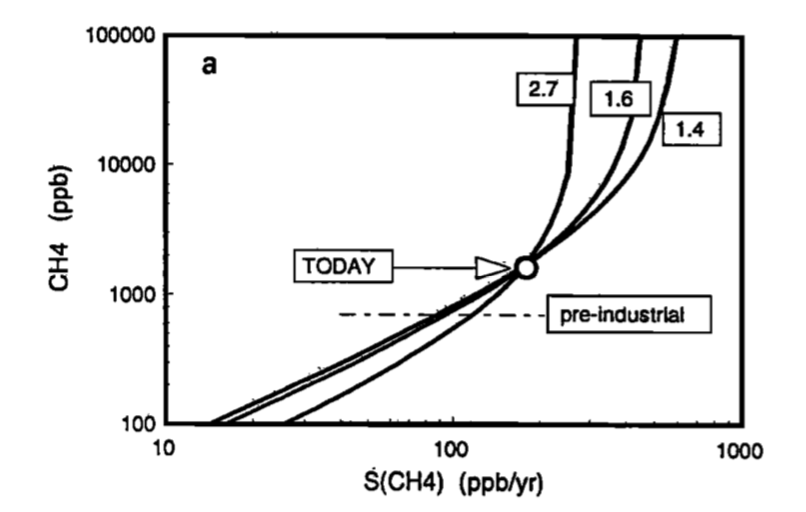
\includegraphics[scale=0.35]{1996-fig1a.png} & 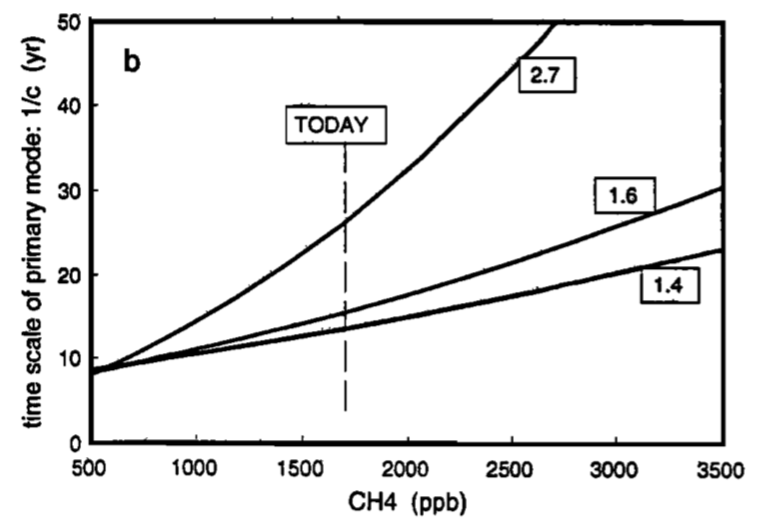
\includegraphics[scale=0.35]{1996-fig1b.png} 
  \end{tabular}
  CH4 concentrations as a function of emission (left) and CH4 lifetime as a function of concentration. The system behaves nonlinearly at higher concentrations.
}

% Slide 9
\frame{\frametitle{Forward Model Test with Variable Lifetime}
  \begin{center}
    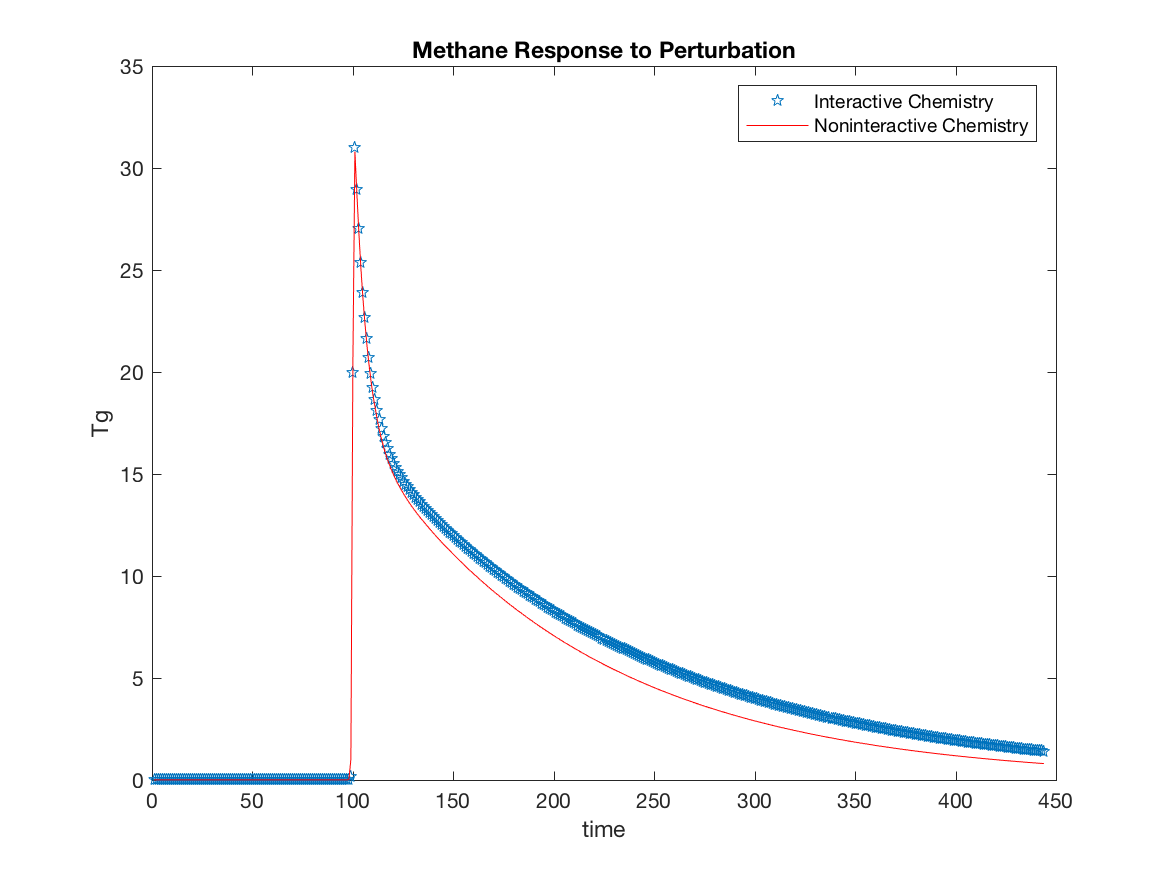
\includegraphics[scale=0.35]{forward_model_test.png} \\
  \end{center}
  A test of our forward model by adding a large methane perturbation. The perturbation decays with a 13 year lifetime in the interactive chemistry case as compared to a 9 year lifetime in a noninteractive case.

}

% Slide 10
\frame{\frametitle{Our Questions}
  \begin{itemize}
  \item What is the effect of adding interactive chemistry (variable OH) on methane emissions estimates?
  \item What is the effect of adding CO+OH chemistry to our inversion?
  \end{itemize}
}

% Slide 11
\frame{\frametitle{Difference Between Interactive and Noninteractive OH}
  \begin{center}
    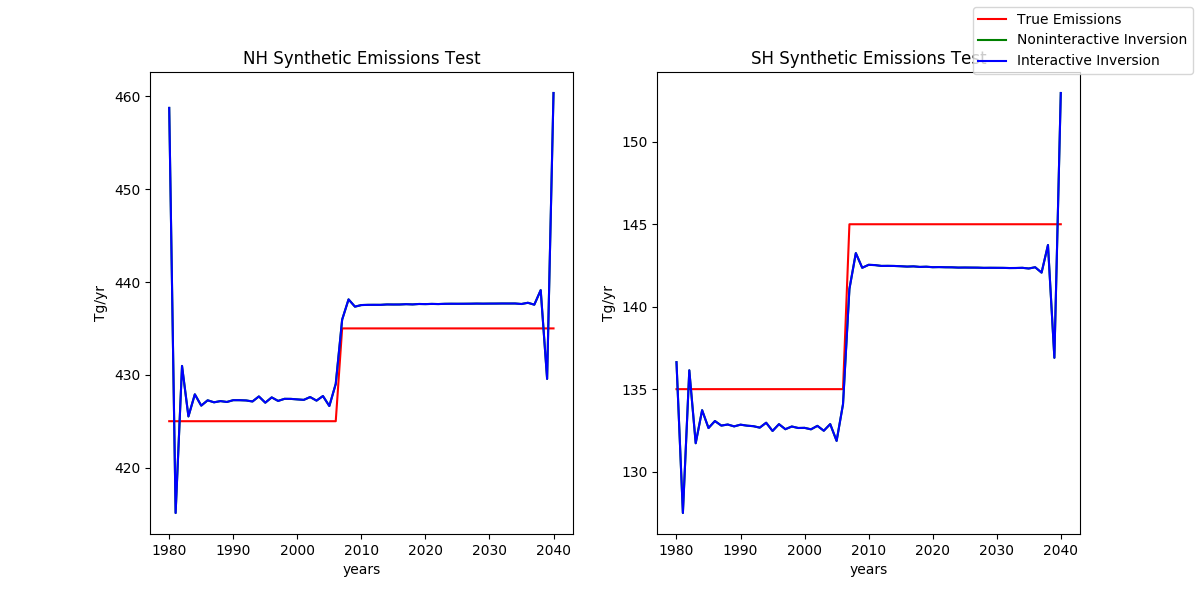
\includegraphics[width=\textwidth]{synthetic_emissions_test.png} \\
  \end{center}
  \begin{itemize}
  \item A test of our inverse model by prescribing synthetic emissions (red dotted line)
  \item Ran inversion with and without interactive OH chemistry
  \end{itemize}
}

% slide 12
\frame{\frametitle{Adding Interactive OH}
  % \begin{center} 
  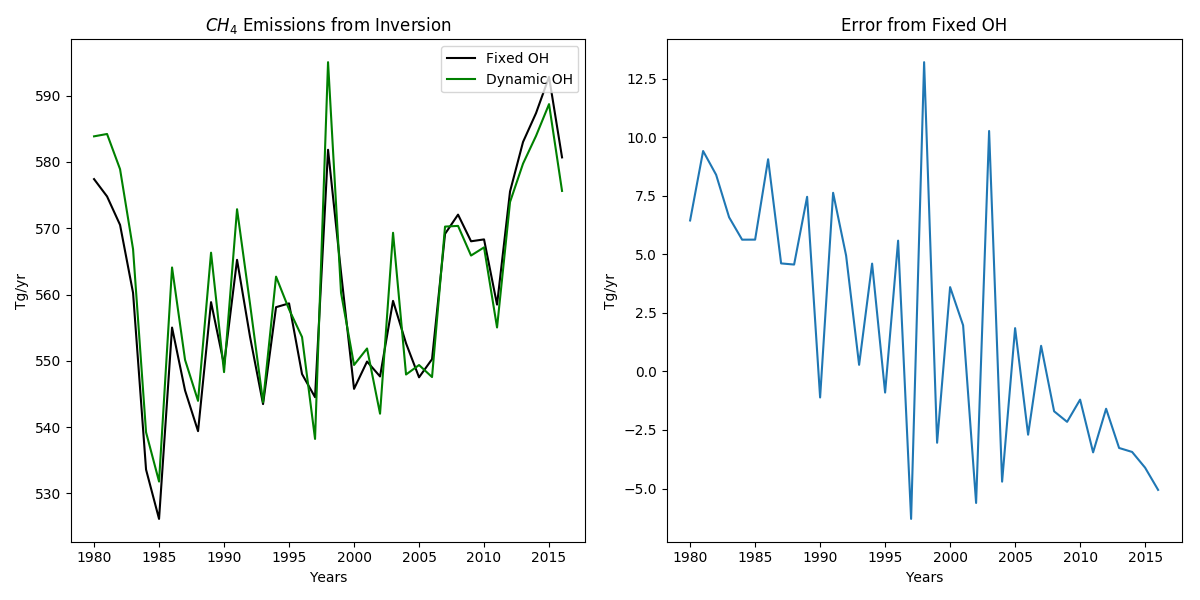
\includegraphics[width=\textwidth]{OH_variability_bias.png} \\
  Results from inversion for both interactive and noninteractive OH chemistry. The trend is due to OH decreasing into the the 21st century.
  % \end{center}
}

% Slide 13
\frame{\frametitle{Effects of Including CO}
  % \begin{center} 
  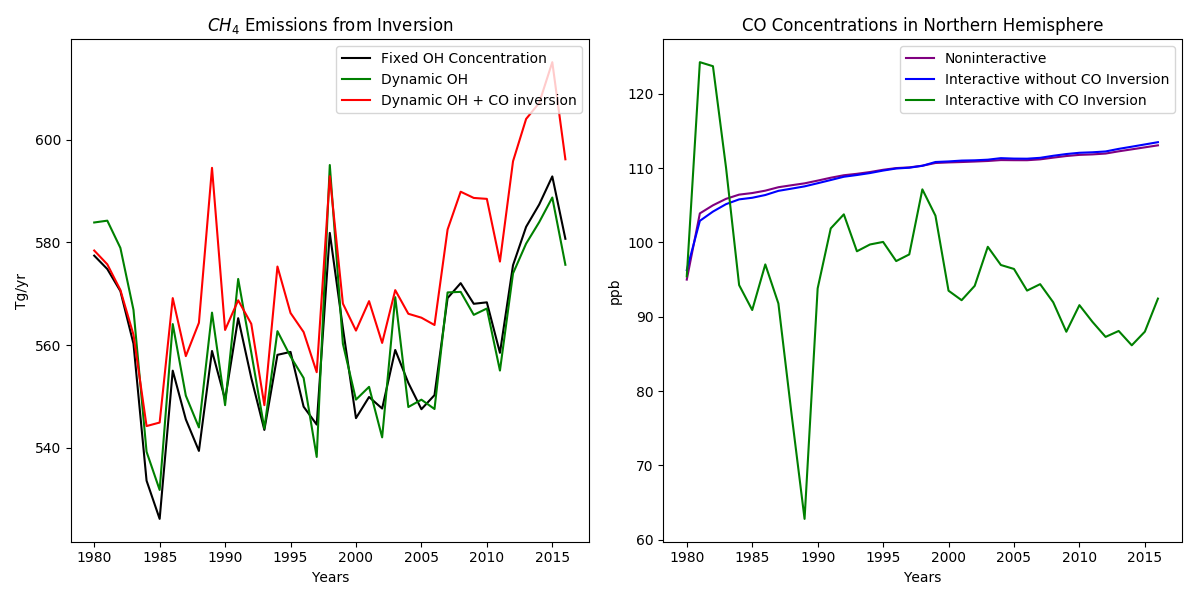
\includegraphics[width=\textwidth]{CO_bias.png} \\
  Methane emissions estimates with the inclusion of CO (left) and CO concentrations for each run in the northern hemisphere (right).
  % \end{center}
}

% Slide 14
\frame{\frametitle{Key Conclusions}
  \begin{itemize}
  \item Methane emissions estimates are biased to higher values when not accounting for interactive OH chemistry
  \item Methane emissions estimates are highly sensitive to CO concentrations
  \end{itemize}
}

%%% End of Main Slides
% Begin Hidden Slides 

% slide 15
\frame{\frametitle{Mathematical formulation}
  \begin{align*}
    \frac{d[CH_4]}{dt} = SCH_4 - R_1 \\
    \frac{d[CO]}{dt} = SCO + R_1 - R_2 \\
    \frac{d[OH]}{dt} = SOH - R_1 - R_2 - R_3 
  \end{align*}

  \begin{itemize}
  \item Let $\mathbf{A}(V)$ be the matrix that represents the differential equation above
  \item Let $V$ be the vector of concentrations of species  and $\delta V$ be a purturbation \\
    $$ \begin{matrix}
      [CH_4] && [CO] && [OH]
    \end{matrix} $$
  \end{itemize}
  \pause
  \begin{align*}
    \frac{dV}{dt}=\mathbf{A}(V)
  \end{align*}
}

\frame{\frametitle{Hartmann-Brodman Theorem}
  Remember Objective: Understand methane nonlinear variability \\
  \pause
  \textbf{Hartmann-Grodman Theorem} \\
  A dynamical system near it's equalibrium point can be accurately represented by a linear Taylor Expansion in the neighborhood of its equalibrium. Additionally, from the expansion, Eigenvalues of the Jacobian correspond to the stability of the system and the Eigenvectors correspond to the modes of the system.
}

\frame{\frametitle{Derivation}
  \begin{equation*}
    \frac{dV}{dt}=\mathbf{A}(V) 
  \end{equation*}
  \begin{equation*}
    \frac{d(V+\delta V)}{dt} = \frac{dV}{dt} + \frac{d\delta V}{dt} = \mathbf{A}(V + \delta V) = \mathbf{A}(V) + J\delta V 
  \end{equation*}
  \begin{itemize}
  \item $\mathbf{J}$ is the Jacobian Matrix
  \item Eigenvalues of $\mathbf{J}$ correspond to inverse of species lifetimes
  \item Eigenvectors correspond to modes
  \end{itemize}
  \begin{equation*}
    \mathbf{J} = 
    \begin{matrix}
      \frac{\partial (d[CH_4]/dt)}{\partial [CH_4]} && \frac{\partial (d[CH_4]/dt)}{\partial [CO]} && \frac{\partial (d[CH_4]/dt)}{\partial [OH]} \\
      % Row 2
      \frac{\partial (d[CO]/dt)}{\partial [CH_4]} && \frac{\partial (d[CO]/dt)}{\partial [CO]} && \frac{\partial (d[CO]/dt)}{\partial [OH]} \\
      % third row
      \frac{\partial (d[OH]/dt)}{\partial d[CH_4]} && \frac{\partial (d[OH]/dt)}{\partial [CO]} && \frac{\partial (d[OH]/dt)}{\partial [OH]}
    \end{matrix}
  \end{equation*}

}
\frame{\frametitle{Methane Lifetime}
  \begin{center}
    \begin{tabular}{lp{5cm}}
      \includegraphics[scale=0.4]{1994-fig2.png} 
      &
        \includegraphics[scale=0.4]{1994-fig4.png} 
    \end{tabular}
  \end{center}
  \begin{itemize}
  \item Left: Methane lifetime $1/e_1$ as a function of E, excess OH. \\
  \item Right: OH lifetime as a function of reaction rate
  \end{itemize}
}

\end{document}

